%%%%%%%%%%%%%%%%%%%%%%%%%%%%%%%%%%%%%%%%%%%%%%%%%%%
%% P3: Phenomenology of Particle Physics                         
%%
%% Author:  André Rubbia                   		 
%%
%% Figure 13.5 Measurements of $R_{\mu\mu}$ from CELLO, MARK Jat PETRA,
%% MAC at PEP, and AMY at TRISTAN as a function of the center-of-mass energy squared $s$. 
%%
%% This work is licensed under the Creative Commons Attribution 4.0 International License. 
%% To view a copy of this license, visit http://creativecommons.org/licenses/by/4.0/ or 
%% send a letter to Creative Commons, PO Box 1866, Mountain View, CA 94042, USA.
%%
%%%%%%%%%%%%%%%%%%%%%%%%%%%%%%%%%%%%%%%%%%%%%%%%%%%

\documentclass[a4paper,10pt]{article}

\usepackage[T1]{fontenc}
\usepackage[utf8]{inputenc}
\usepackage{lmodern}
\usepackage[labelfont=bf]{caption}
\usepackage{upgreek}

\usepackage{tikz}
\usepackage{pgfplots}
\pgfplotsset{compat=1.17}
\usepgfplotslibrary{ternary}
\usepgfplotslibrary{fillbetween}
\usepgfplotslibrary{external}

\usepackage{braket}

\def\d{\mathrm{d}}

\pgfkeys{/pgf/number format/.cd,1000 sep={}}

\begin{document}

%%%%%%%%%%%%%%%%% FIGURE %%%%%%%%%%%%%%%%%%%%%%%%%%%%%%%%%%
\begin{figure}[htb]
\begin{center}
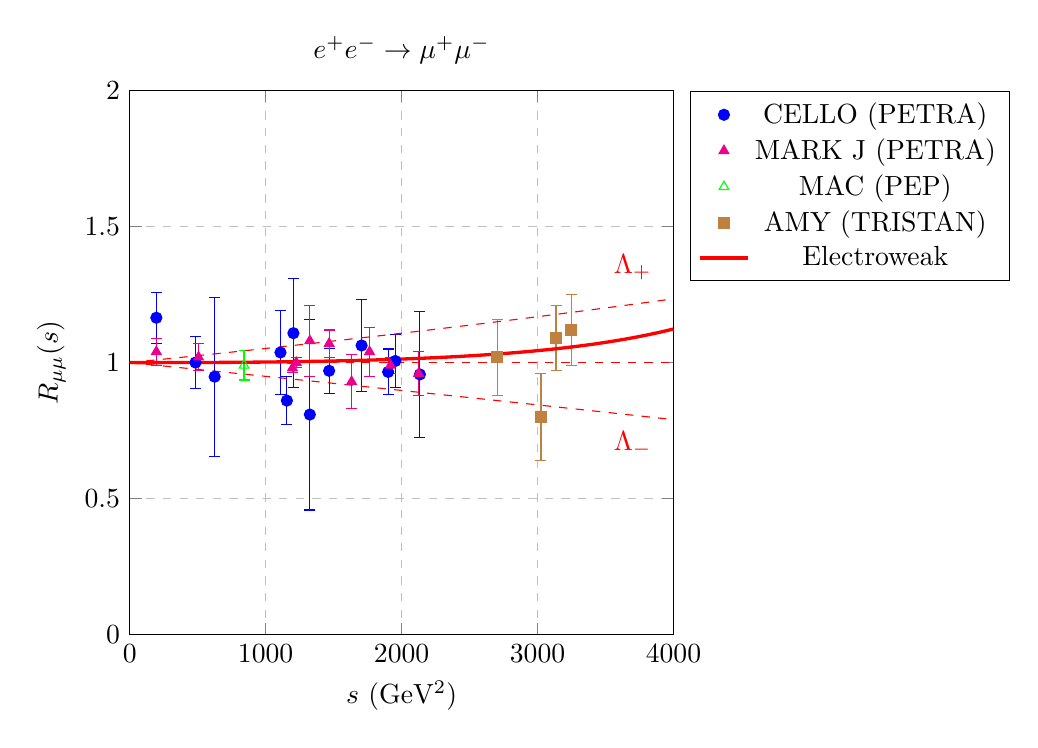
\begin{tikzpicture}[scale=1.]
\begin{axis}[
    width=0.7\textwidth,
    height=0.7\textwidth,
    title={$e^+e^-\rightarrow \mu^+\mu^-$},
    xlabel={$s$~(GeV$^2$)},
    ylabel={$R_{\mu\mu}(s)$},
    xmin=0, xmax=4000,
    ymin=0.0, ymax=2,
	legend style={legend pos = outer north east},
    	ymajorgrids=true,
    	xmajorgrids=true,
    grid style=dashed,
]

%% CELLO R_mumu
\addplot[
    color=blue,
    only marks,
    error bars/.cd,
    y dir=both, y explicit
    ]
    coordinates {
( 196.0 , 1.1649537847454785 )+-(0, 0.09408710150339811 )
( 484.0 , 1.0001628613741498 )+-(0, 0.09448119427829925 )
( 625.0 , 0.94813180674401 )+-(0, 0.29285420947591795 )
( 1108.8899999999999 , 1.0371639664625136 )+-(0, 0.1538423329847326 )
( 1156.0 , 0.8601877942148093 )+-(0, 0.08801776455621982 )
( 1204.0900000000001 , 1.10817577611995 )+-(0, 0.2003480675041567 )
( 1324.9599999999998 , 0.8088752751911046 )+-(0, 0.3508875995408928 )
( 1466.8899999999999 , 0.9698674051705023 )+-(0, 0.08342383201263331 )
( 1705.6899999999998 , 1.0629192981890334 )+-(0, 0.1690276745235391 )
( 1900.96 , 0.965638319760072 )+-(0, 0.08417556096721353 )
( 1953.6400000000003 , 1.005900410810671 )+-(0, 0.09723182913691601 )
( 2134.44 , 0.9563931923404347 )+-(0, 0.2320184929469682 )
};

%% MarkJ R_mumu
\addplot[
    color=magenta,
    only marks,
    mark = triangle*,
    error bars/.cd,
    y dir=both, y explicit
    ]
    coordinates {
    % 14 GeV
 ( 196 , 1.04 )+-(0, 0.05 )
   % 22.5
( 506.25 , 1.02 )+-(0, 0.05 )
  % 34.6
  ( 1197.16 , 0.98 )+-(0, 0.016 )
  % 35.0
  ( 1225.0, 1.00 )+-(0, 0.018)
  % 36.4
  ( 1325.0,  1.08)+-(0, 0.13)
  % 38.3
  ( 1467, 1.07)+-(0, 0.05)
  % 40.4
  ( 1632, 0.93)+-(0, 0.10)
  % 42.0
  ( 1764, 1.04)+-(0, 0.09)
  % 43.8
  (  1918, 0.99)+-(0, 0.03)
  % 46.1
  ( 2125, 0.96)+-(0, 0.08)
%( 1584.0399999999997 , 1.01 )+-(0, 0.06403124237432849 )
%( 1989.16 , 0.99 )+-(0, 0.0565685424949238 )
};

%% PEP MAC R_mumu
\addplot[
    color=green,
    only marks,
    mark = triangle,
    error bars/.cd,
    y dir=both, y explicit
    ]
    coordinates {( 841 , 0.99 )+-(0, 0.05385164807134505 )
};


%% AMY R_mumu Phys.Lett.B 218 (1989) 112-118
\addplot[
    color=brown,
    only marks,
    mark = square*,
    error bars/.cd,
    y dir=both, y explicit
    ]
    coordinates {
% 52
( 2704.0 , 1.02 )+-(0, 0.14 )
% 55
( 3025.0 , 0.80 )+-(0, 0.16 )
% 56
( 3136.0 , 1.09 )+-(0, 0.12 )
% 57
( 3249.0 , 1.12 )+-(0, 0.13 )
};

\addplot[very thick,
    color=red,
    no marks
    ]
    coordinates {
( 0, 1.0 )
( 50, 0.9999761725466781 )
( 100, 0.9999626713192045 )
( 150, 0.9999598919550471 )
( 200, 0.9999682452003099 )
( 250, 0.9999881575533657 )
( 300, 1.0000200719395025 )
( 350, 1.0000644484182704 )
( 400, 1.0001217649253105 )
( 450, 1.000192518050566 )
( 500, 1.0002772238548847 )
( 550, 1.0003764187271467 )
( 600, 1.0004906602841903 )
( 650, 1.0006205283159475 )
( 700, 1.0007666257783465 )
( 750, 1.0009295798367144 )
( 800, 1.001110042962574 )
( 850, 1.0013086940869274 )
( 900, 1.0015262398133047 )
( 950, 1.0017634156940867 )
( 1000, 1.0020209875738244 )
( 1050, 1.0022997530035382 )
( 1100, 1.00260054273023 )
( 1150, 1.0029242222661419 )
( 1200, 1.0032716935425827 )
( 1250, 1.0036438966534884 )
( 1300, 1.0040418116942194 )
( 1350, 1.0044664607014917 )
( 1400, 1.0049189097007352 )
( 1450, 1.0054002708676213 )
( 1500, 1.0059117048109738 )
( 1550, 1.0064544229847816 )
( 1600, 1.0070296902375993 )
( 1650, 1.0076388275081967 )
( 1700, 1.008283214676983 )
( 1750, 1.0089642935834058 )
( 1800, 1.0096835712202954 )
( 1850, 1.0104426231169235 )
( 1900, 1.0112430969234354 )
( 1950, 1.0120867162102627 )
( 2000, 1.0129752844971591 )
( 2050, 1.0139106895276264 )
( 2100, 1.0148949078057055 )
( 2150, 1.0159300094134383 )
( 2200, 1.017018163128737 )
( 2250, 1.018161641864956 )
( 2300, 1.019362828455168 )
( 2350, 1.0206242218059878 )
( 2400, 1.0219484434478063 )
( 2450, 1.0233382445104968 )
( 2500, 1.024796513156048 )
( 2550, 1.0263262825022037 )
( 2600, 1.0279307390740486 )
( 2650, 1.029613231823603 )
( 2700, 1.031377281760929 )
( 2750, 1.0332265922439898 )
( 2800, 1.0351650599786246 )
( 2850, 1.0371967867845129 )
( 2900, 1.0393260921879601 )
( 2950, 1.0415575269077795 )
( 3000, 1.0438958873065398 )
( 3050, 1.0463462308860447 )
( 3100, 1.0489138929131747 )
( 3150, 1.051604504270241 )
( 3200, 1.0544240106328546 )
( 3250, 1.0573786930880837 )
( 3300, 1.0604751903165017 )
( 3350, 1.0637205224736948 )
( 3400, 1.0671221169200764 )
( 3450, 1.0706878359625855 )
( 3500, 1.074426006788195 )
( 3550, 1.0783454537873505 )
( 3600, 1.0824555334856936 )
( 3650, 1.086766172324986 )
( 3700, 1.0912879075593074 )
( 3750, 1.0960319315607094 )
( 3800, 1.1010101398599315 )
( 3850, 1.1062351832829709 )
( 3900, 1.1117205245837436 )
( 3950, 1.1174805000173473 )
( 4000, 1.1235303863481956 )
};

       \addplot [red,dashed, domain=0:4000, samples=75] {(1+(x/(x-40000)))^2};
      \addplot [red,dashed, domain=0:4000, samples=75] {(1-(x/(x-40000)))^2};
      \addplot [red,domain=0:4000, samples=75, dashed] {1};

    \legend{CELLO (PETRA),
     MARK J (PETRA),
     MAC (PEP),
     AMY (TRISTAN),
     Electroweak
 	}
\node[red] at (axis cs:3700,1.35) {$\Lambda_+$};
\node[red] at (axis cs:3700,0.7) {$\Lambda_-$};
\end{axis}

\end{tikzpicture}
\caption{Measurements of $R_{\mu\mu}$ from CELLO, MARK Jat PETRA,
MAC at PEP, and AMY at TRISTAN as a function of the
center-of-mass energy squared $s$. The error bars include statistical and systematic errors.
The solid line labeled ``Electroweak'' shows the electroweak prediction. The horizontal dashed line
is the QED prediction.
The dashed curves labeled $\Lambda_\pm$ show the deviation from QED for cutoff parameters $\Lambda_\pm$ = 200~GeV
(see Section 13.6 of the book). }
\end{center}
\end{figure}
%%%%%%%%%%%%%%%%% END FIGURE %%%%%%%%%%%%%%%%%%%%%%%%%%%%%%
%

\end{document}
